\documentclass{beamer}

\usepackage{beamerthemesplit}
\usepackage{verbatim}
\usepackage[normalem]{ulem}

\usepackage{xcolor}

\definecolor{gold}{rgb}{1.,0.84,0.}
\definecolor{brightred}{rgb}{1.,0.4,0.4}
\definecolor{mygray}{RGB}{200,200,200}
\definecolor{lightsteelblue}{RGB}{176,196,222}
\definecolor{lightskyblue}{RGB}{135,206,250}
\definecolor{cadetblue}{RGB}{95,158,160}

\usetheme{default}
\usecolortheme{mule}

\usefonttheme{serif}

%\DeclareGraphicsExtensions{.pdf,.png,.jpg}

\newcommand{\snr}{$S/N$}
\newcommand{\snT}{$(S/N)_{\textrm{size}}$}
%\newcommand{\snT}{$\left( \frac{S}{N}\right)_{\textrm{size}}$}
\newcommand{\snflux}{$(S/N)_{\textrm{flux}}$}
%\newcommand{\snflux}{$\left( \frac{S}{N}\right)_{\textrm{flux}}$}

\newcommand{\lensfit}{\texttt{LENSFIT}}
\newcommand{\numba}{\texttt{Numba}}
\newcommand{\python}{\texttt{Python}}
\newcommand{\ngmix}{\texttt{ngmix}}
\newcommand{\shear}{{\bf g}}
\newcommand{\redmapper}{redMaPPer}
\newcommand{\est}{$e$}
\newcommand{\mest}{e}


\newcommand{\mcal}{metacalibration}
\newcommand{\Mcal}{Metacalibration}

\newcommand{\mcalR}{$R$}
\newcommand{\mcalRpsf}{$R^{p}$}
\newcommand{\mcalRS}{$R_{S}$}

\newcommand{\prelim}{{\bf{\it Preliminary}}}



\title{Metacalibration Update}
\author{Erin Sheldon}
\institute{Brookhaven National Laboratory}

% http://texblog.net/latex-archive/plaintex/beamer-footline-frame-number/
% to add the page (frame ) number and not screw up the bottom line
% works for split themes?
\expandafter\def\expandafter\insertshorttitle\expandafter{%
      \insertshorttitle\hfill%
        \insertframenumber\,/\,\inserttotalframenumber}

% suppress navigation bar
\beamertemplatenavigationsymbolsempty
\setbeamertemplate{footline}{}

\begin{document}

\frame{\titlepage}


\setbeamertemplate{background canvas}[vertical shading][bottom=mgray,top=mblack]

\setbeamerfont*{itemize/enumerate body}{size=\Large}
\setbeamerfont*{itemize/enumerate subbody}{parent=itemize/enumerate body}
\setbeamerfont*{itemize/enumerate subsubbody}{parent=itemize/enumerate body}


\frame
{
    \frametitle{Metacal Update}

    \begin{itemize}

        \item See previous talks showing \mcal\ works well in simulations

        \item Y1 $r,i,z$ measurements
        \item Y3 $r,i,z$ measurements
        \item Now have formalism for response and selection effects in
            shear-shear correlations.

    \end{itemize}
}

{

    \setbeamertemplate{background canvas}[vertical shading][bottom=white,top=white]
    \frame
    {
        \frametitle{New Y1 $r,i,z$ measurements}

                \begin{center}
                    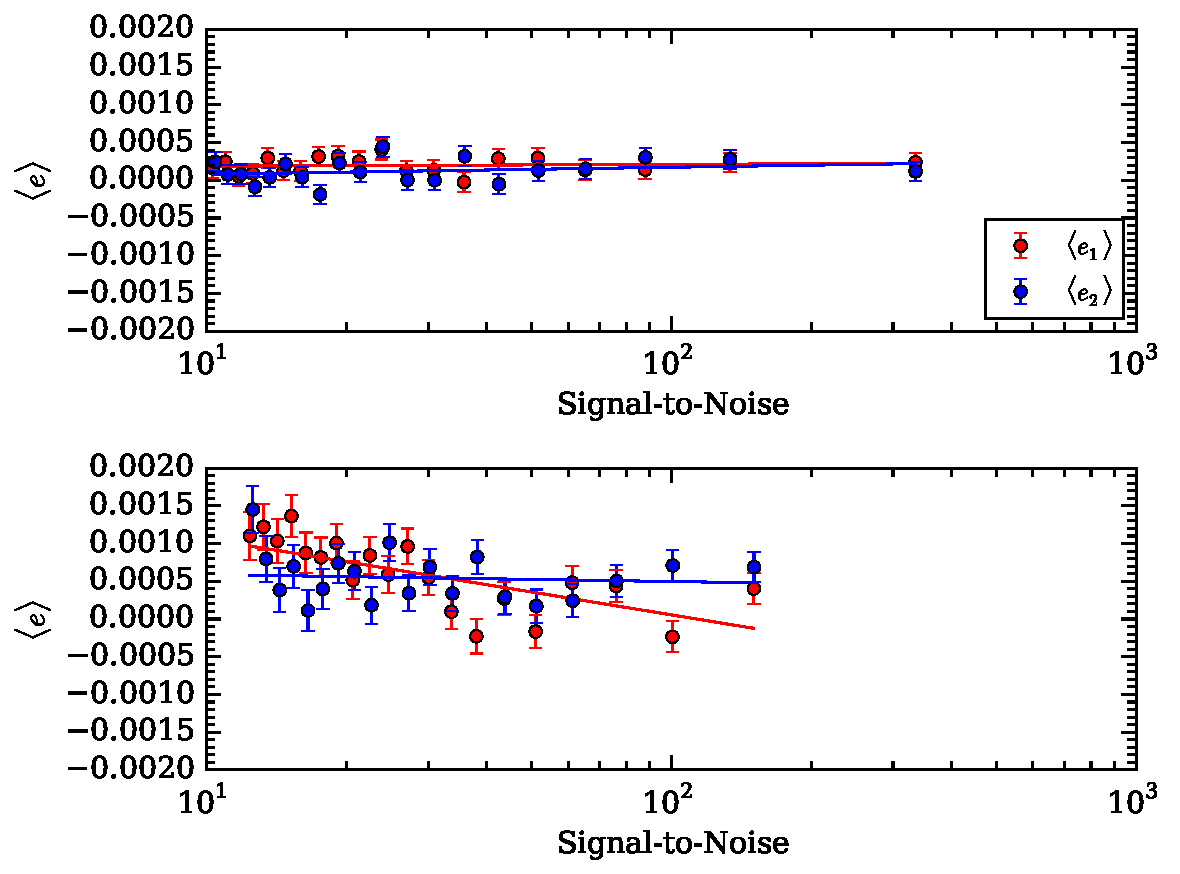
\includegraphics[width=0.8\textwidth]{lin_split_snr.pdf}
                \end{center}

        \vspace{5mm}
        Top \texttt{metacal}, bottom \texttt{im3shape}. Plot Michael Troxel


    }
    \setbeamertemplate{background canvas}[vertical shading][bottom=mgray,top=mblack]
}
{
    \setbeamertemplate{background canvas}[vertical shading][bottom=white,top=white]
    \frame
    {
        \frametitle{New Y1 $r,i,z$ measurements}

                \begin{center}
                    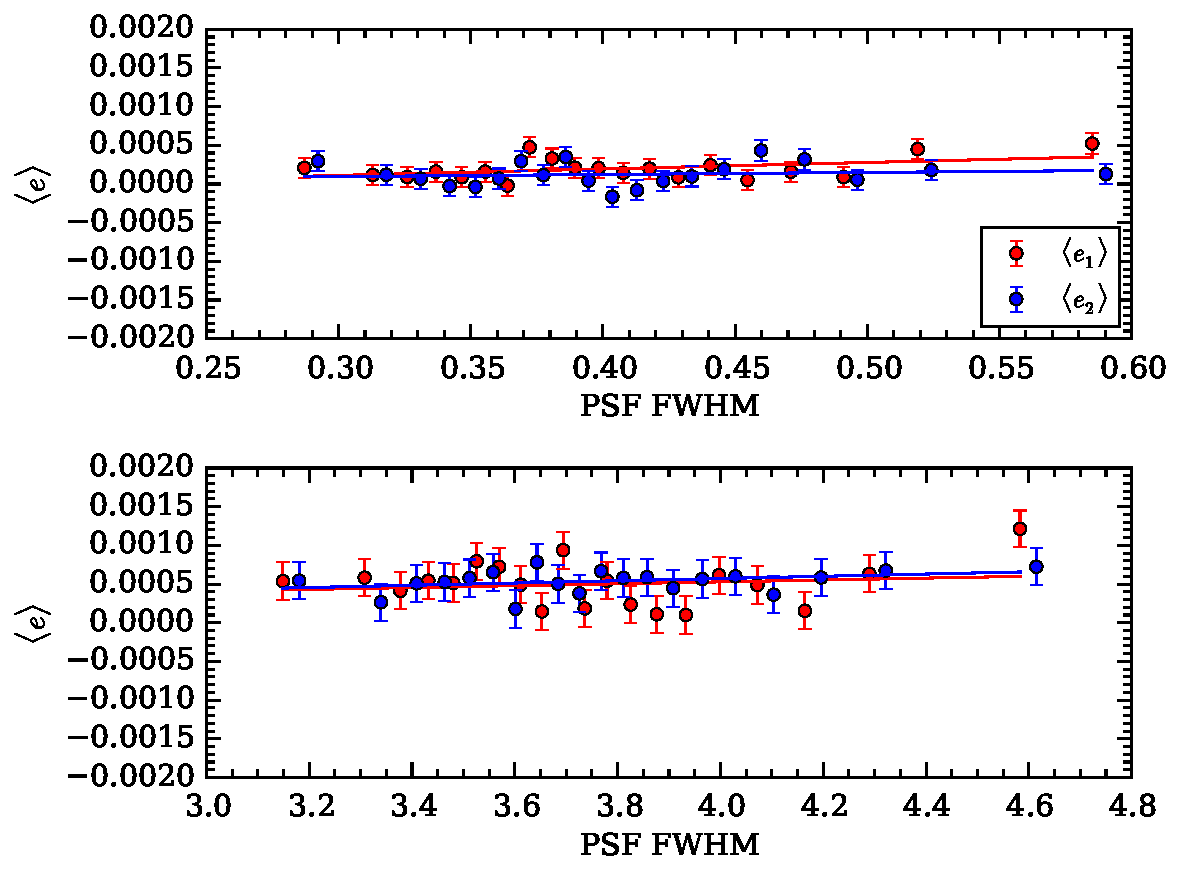
\includegraphics[width=0.8\textwidth]{lin_split_psfsize.pdf}
                \end{center}

        \vspace{5mm}
        Top \texttt{metacal}, bottom \texttt{im3shape}. Plot Michael Troxel


    }
    \setbeamertemplate{background canvas}[vertical shading][bottom=mgray,top=mblack]
}


{
    \setbeamertemplate{background canvas}[vertical shading][bottom=white,top=white]
    \frame
    {
        \frametitle{New Y1 $r,i,z$ measurements}

                \begin{center}
                    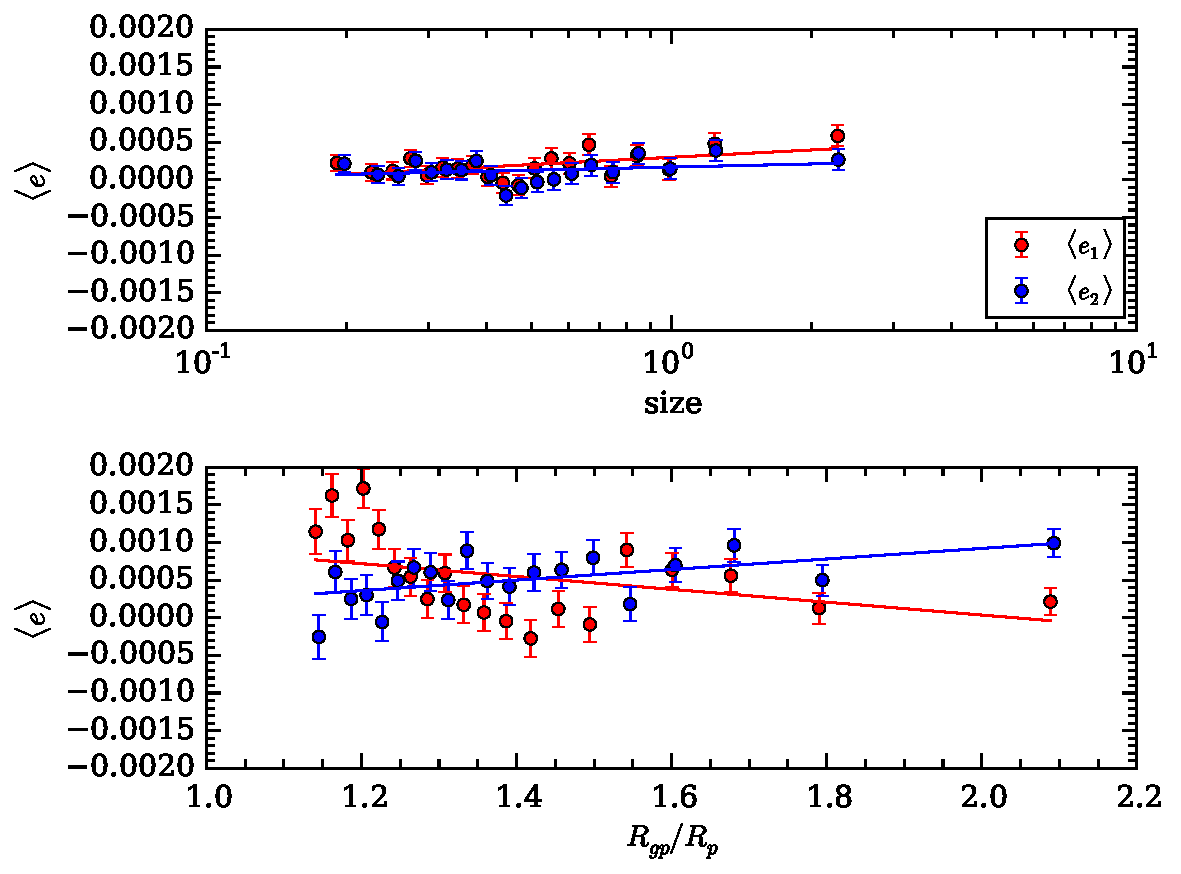
\includegraphics[width=0.8\textwidth]{lin_split_radius.pdf}
                \end{center}

        \vspace{5mm}
        Top \texttt{metacal}, bottom \texttt{im3shape}. Plot Michael Troxel


    }
    \setbeamertemplate{background canvas}[vertical shading][bottom=mgray,top=mblack]
}

{
    \setbeamertemplate{background canvas}[vertical shading][bottom=white,top=white]
    \frame
    {
        \frametitle{New Y1 $r,i,z$ measurements}

        \begin{columns}
            \begin{column}{0.5\textwidth}
                \begin{center}
                    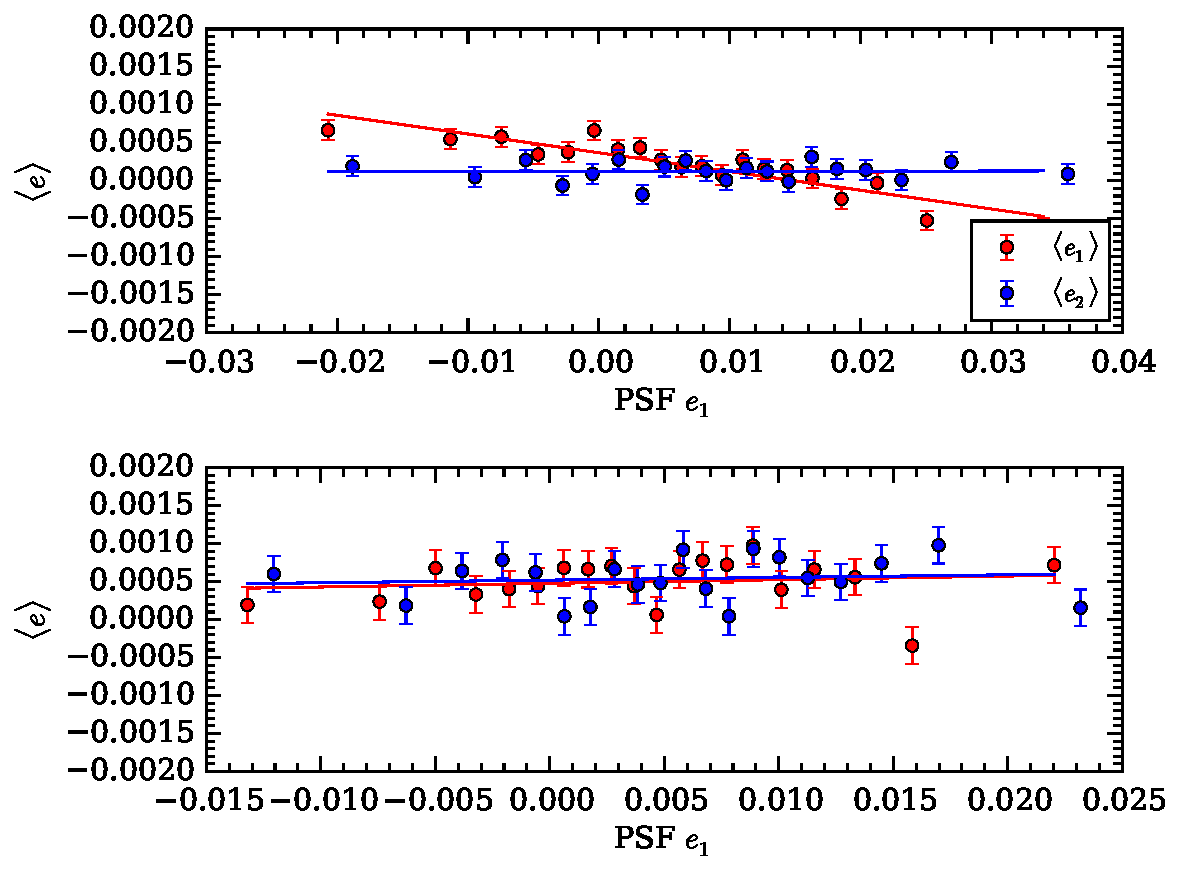
\includegraphics[width=\textwidth]{lin_split_psf1.pdf}
                \end{center}
            \end{column}
            \begin{column}{0.5\textwidth}
                \begin{center}
                    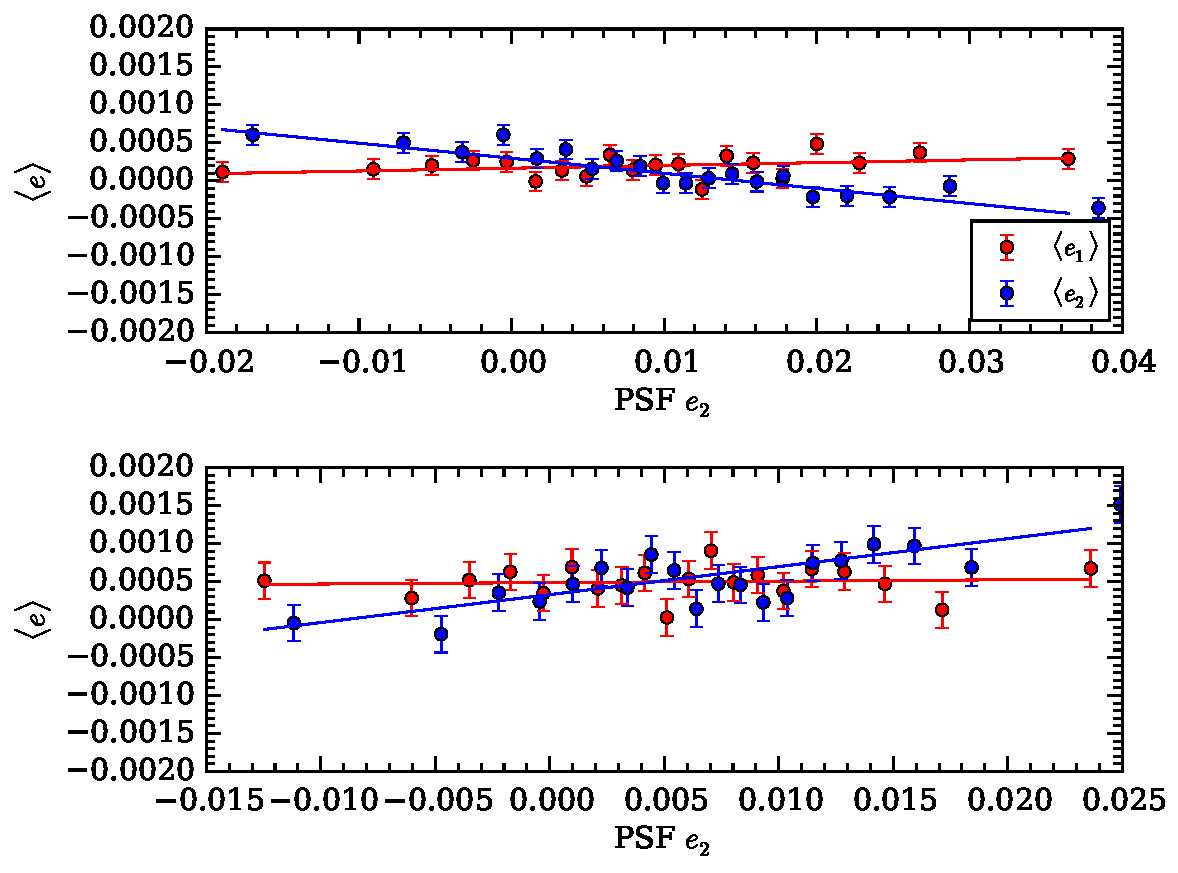
\includegraphics[width=\textwidth]{lin_split_psf2.pdf}
                \end{center}
            \end{column}

        \end{columns}

        \vspace{5mm}
        Top \texttt{metacal}, bottom \texttt{im3shape}. Plot Michael Troxel


    }
    \setbeamertemplate{background canvas}[vertical shading][bottom=mgray,top=mblack]
}

\frame
{
    \frametitle{Y1 Metacal Update}

    \begin{itemize}

        \item These $r,i,z$ measurements are an improvement over $r$ only.

        \item More exposures results in reduced correlation between shape
            and shape residuals on individual images.

    \end{itemize}
}

\frame
{
    \frametitle{Y3 Metacal Update}

    \begin{itemize}

        \item 3000 Y3 tiles run.

        \item Expect further improvement due to large number of
            exposures

    \end{itemize}
}

\frame
{
    \frametitle{New Y3 $r,i,z$ measurements}

    \begin{center}
        \includegraphics[width=0.8\textwidth]{{test-001-e-vs-e1psf-s2n-10.0-Tratio-0.50}.pdf}
    \end{center}

    \vspace{3mm}
    $g_1 = (-0.00142 \pm 0.00259) g_1^{psf} + (0.000346 \pm 2.87e-05)$

}

\frame
{
    \frametitle{New Y3 $r,i,z$ measurements}

    \begin{center}
        \includegraphics[width=0.8\textwidth]{{test-001-e-vs-e2psf-s2n-10.0-Tratio-0.50}.pdf}
    \end{center}
    \vspace{3mm}
    $g_2 = (-0.000282 \pm 0.00311) g_2^{psf} + (5.1e-07 \pm 3.3e-05)$

}

\frame
{
    \frametitle{New Y3 $r,i,z$ measurements}

            \begin{center}
                \includegraphics[width=\textwidth]{{test-001-e-vs-s2n-Tratio-0.50}.pdf}
            \end{center}

}

\frame
{
    \frametitle{Response Terms}

    \begin{itemize}

        \item All shear measurements are effectively response weighted.

        \item If we know responses, we can interpret in terms of the
            weighted mean.

        \item I just posted a draft of the math on the \mcal\ channel.

        \item I have verified the results for mean shears (e.g. ggl)

        \item Response for shear 2pt still needs verification


    \end{itemize}
}





\end{document}
